% 附加题第 6 题（本库第 35 题）「Z」字形折线段图：按固定源内容流矢量层精确值复刻。
% 原点取空心点 O 的环心（源页 (471.06, 666.48) pt），y 向上。
% 轴为填充细条（此处以 0.72/0.84 线宽近似）；箭头为填充三角（底宽 6、长 6）。
% 源内瑕疵一律照录：y 轴倾斜 1.67°（底 (472.50,620.16)→顶 (469.62,719.28)）；x 轴中心线高于
% 折线真零位 1.59；各向异性 1.10；x 轴两端伸出不对称；y 轴无刻度（x 轴有 2 条向上刻度）。
% 折线 3 段：A–B（水平）、B–O–C（一条不断开的整线段，过 O 处不中断）、C–D（水平）。
% 五个空心环照源画法：白填充+黑描边（会把轴线/折线在环内擦出白心），直径 ≈2.88。
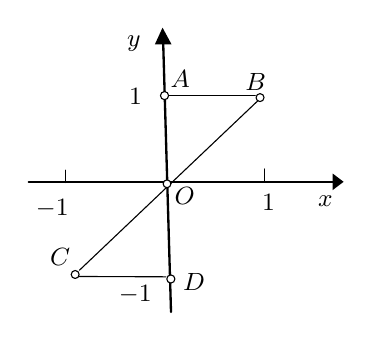
\begin{tikzpicture}[line cap=round,line join=round,font=\small,x=0.03515cm,y=0.03515cm]
% ===== 坐标轴（照源：y 轴带倾斜）=====
\draw[line width=0.72pt] (-49.98,0.72)--(60.18,0.72);  % x 轴主体
\draw[line width=0.84pt] (1.44,-46.32)--(-1.44,52.8);  % y 轴（照源倾斜）
% ===== 轴箭头（填充三角）=====
\fill (63.78,0.72)--(59.82,3.72)--(59.82,-2.28)--cycle;  % x 箭头（尖 534.84；底边 530.88＝清单实测，长 3.96）
\fill (-1.62,56.4)--(-4.38,50.4)--(1.62,50.4)--cycle;  % y 箭头（尖 722.88）
% ===== x 轴刻度（2 条，只向上；y 轴照源无刻度）=====
\draw (-36.78,0.48)--(-36.78,4.92);
\draw (35.16,0.96)--(35.16,5.4);
% ===== 折线（3 段）=====
\draw (0.66,31.8)--(31.86,31.8);   % A–B（水平）
\draw (32.94,30.12)--(-31.62,-31.2);   % B–O–C（整线段）
\draw (-31.62,-33.48)--(-0.42,-33.6);   % C–D（水平）
% ===== 五个空心环（白填充+黑描边，照源层序盖在线之上）=====
\fill[white] (0,0) circle (1.41pt);
\draw (0,0) circle (1.41pt);   % 空心环 O
\fill[white] (-0.9,31.86) circle (1.47pt);
\draw (-0.9,31.86) circle (1.47pt);   % 空心环 A
\fill[white] (33.6,31.14) circle (1.44pt);
\draw (33.6,31.14) circle (1.44pt);   % 空心环 B
\fill[white] (-33.18,-32.76) circle (1.44pt);
\draw (-33.18,-32.76) circle (1.44pt);   % 空心环 C
\fill[white] (1.38,-34.38) circle (1.47pt);
\draw (1.38,-34.38) circle (1.47pt);   % 空心环 D
% ===== 标注（照源基线左端，显式坐标）=====
\node[anchor=base west,inner sep=0] at (-14.58,49.56) {\(y\)};
\node[anchor=base west,inner sep=0] at (54.42,-8.16) {\(x\)};
\node[anchor=base west,inner sep=0] at (2.58,-7.56) {\(O\)};
\node[anchor=base west,inner sep=0] at (1.14,34.8) {\(A\)};
\node[anchor=base west,inner sep=0] at (28.14,33.72) {\(B\)};
\node[anchor=base west,inner sep=0] at (-42.42,-29.64) {\(C\)};
\node[anchor=base west,inner sep=0] at (5.58,-38.64) {\(D\)};
\node[anchor=base west,inner sep=0] at (-13.86,28.56) {\(1\)};
\node[anchor=base west,inner sep=0] at (-17.58,-42.48) {\(-1\)};
\node[anchor=base west,inner sep=0] at (-47.58,-11.28) {\(-1\)};
\node[anchor=base west,inner sep=0] at (34.14,-9.6) {\(1\)};
\end{tikzpicture}
